\begin{apendicesenv}
% \partapendices

\chapter{Detalhamento e Vistas do Projeto Estrutural}
\label{apendice_cad_chassi}

\begin{figure}[htbp]
    \centering
    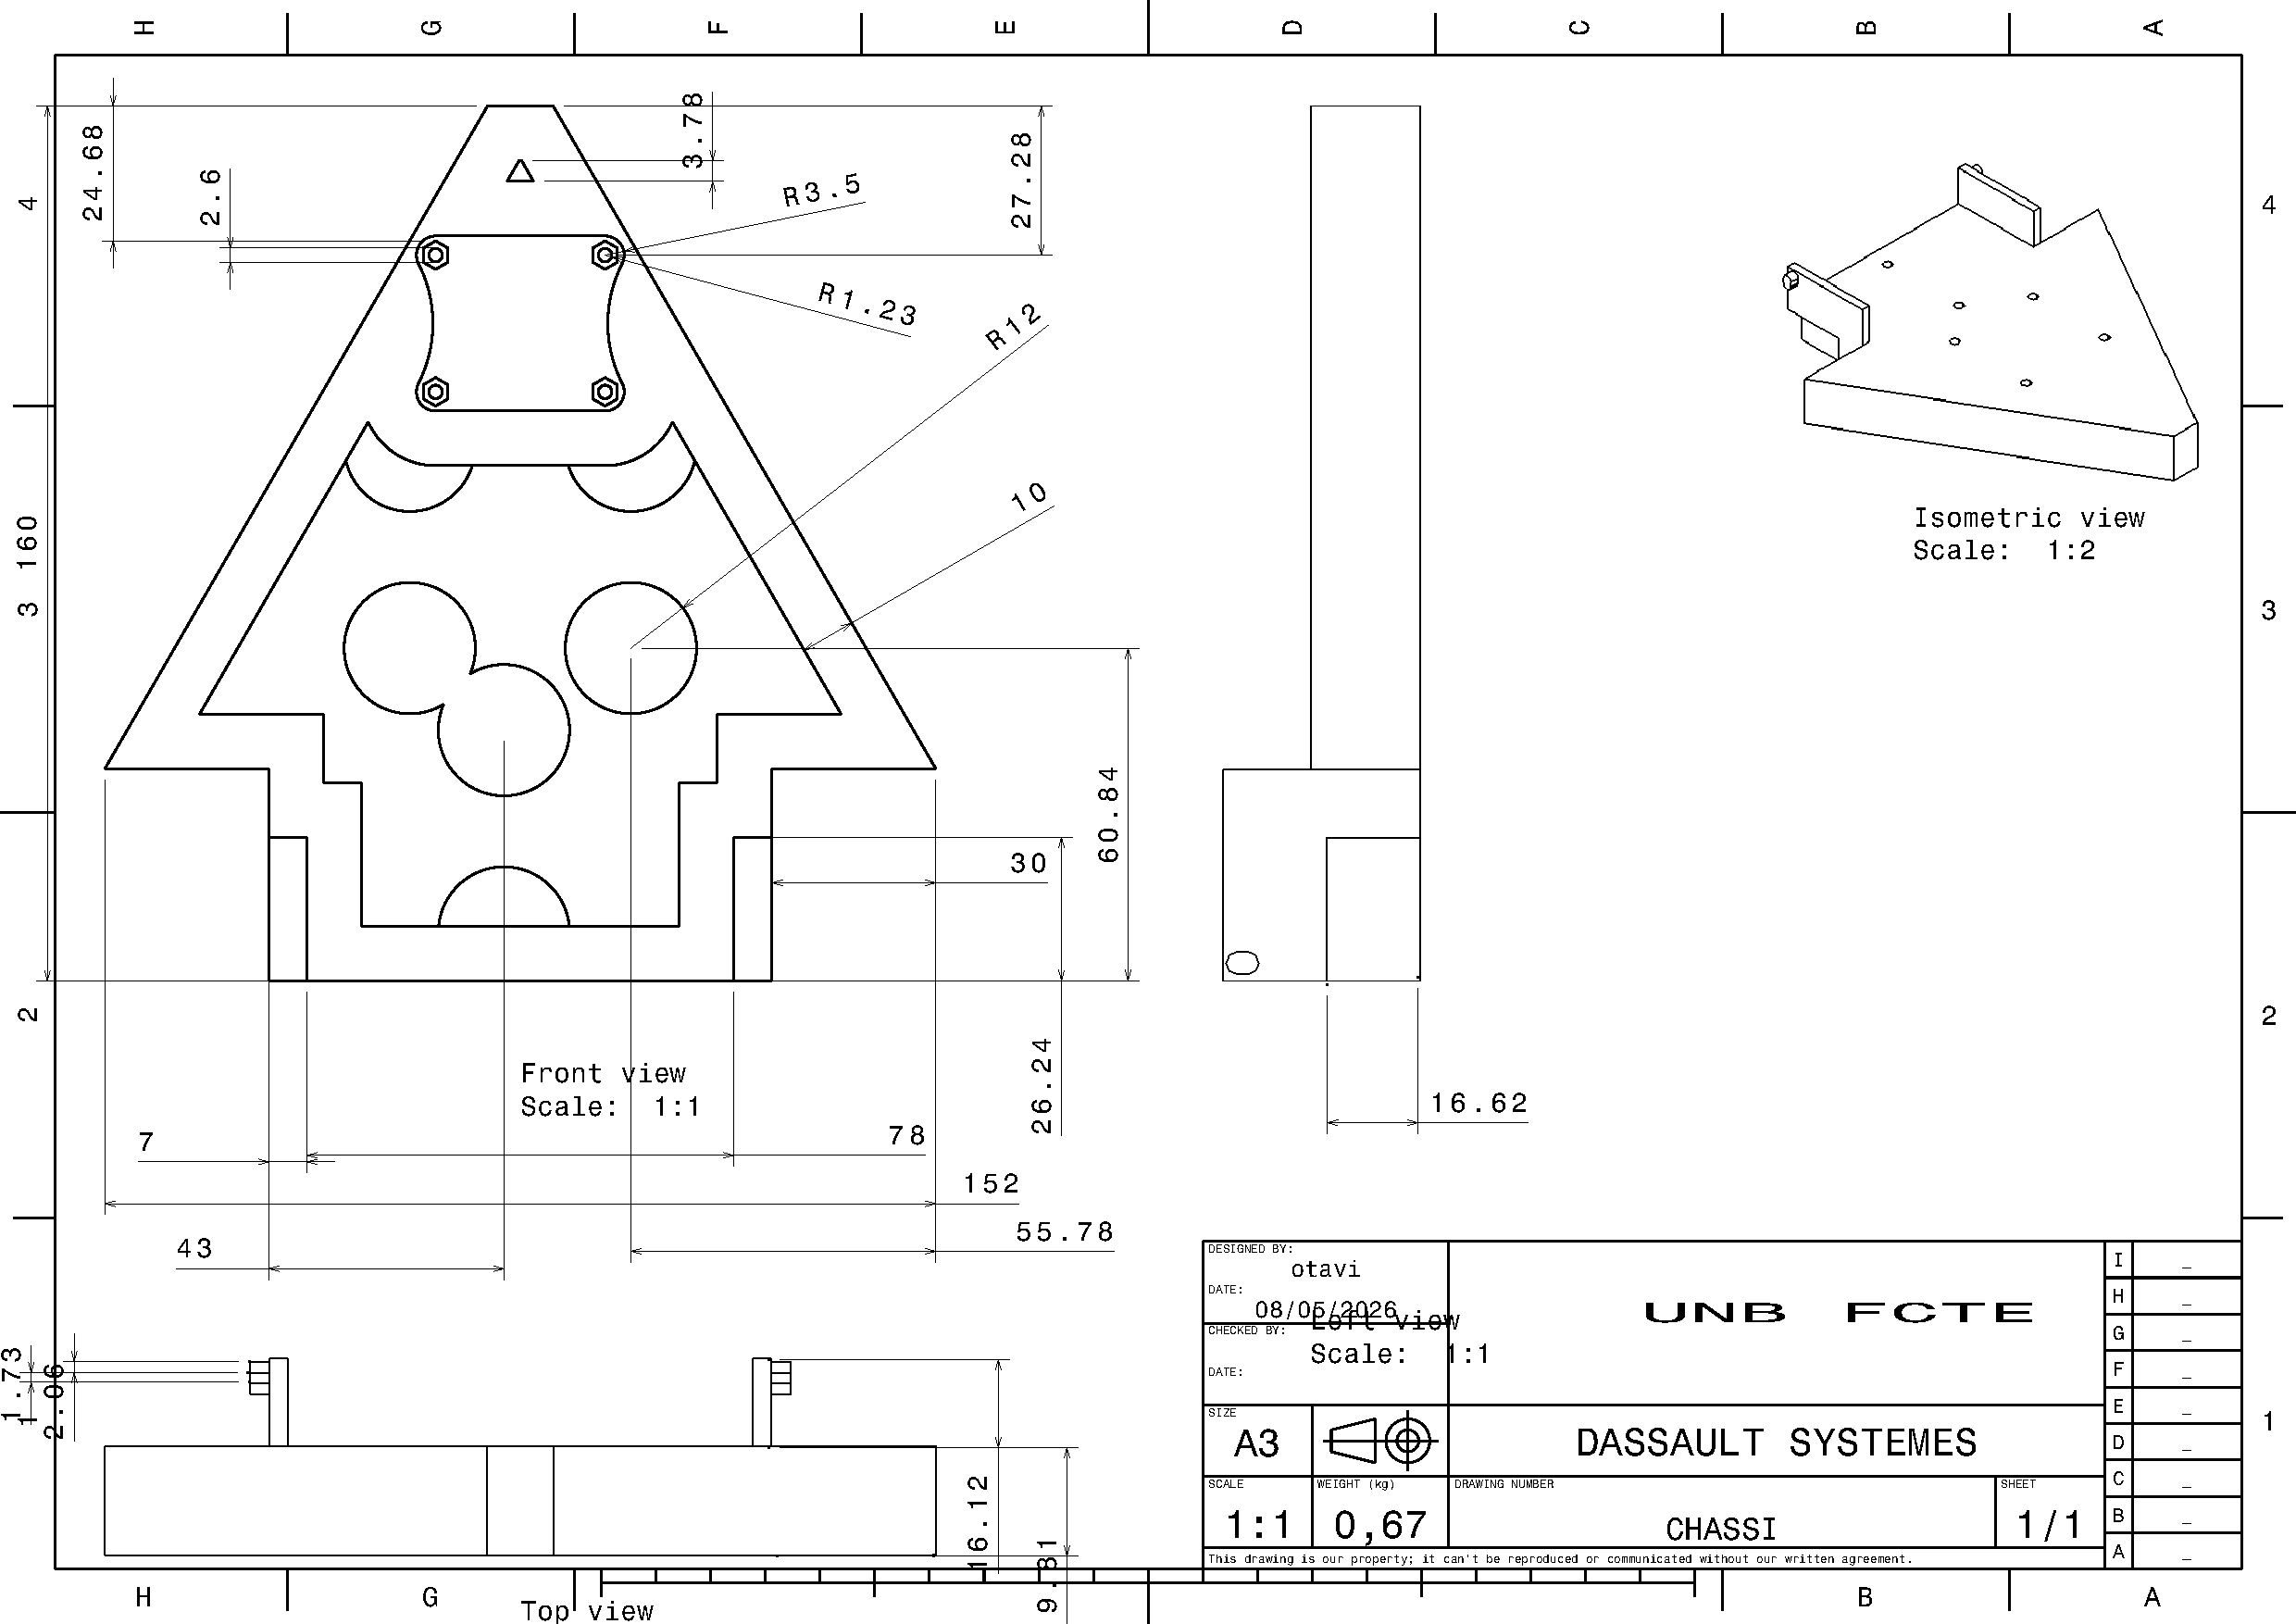
\includegraphics[width=0.55\linewidth]{figuras/CHASSI_1_prototipo_entrega_2.pdf}
    \caption{Prancha técnica do primeiro protótipo: vistas frontal, superior, lateral e isométrica com cotas de fabricação (escala 1:1, peso 0{,}67\,kg).}
    \label{fig:chassi_draw_v1}
\end{figure}

\begin{figure}[htbp]
    \centering
    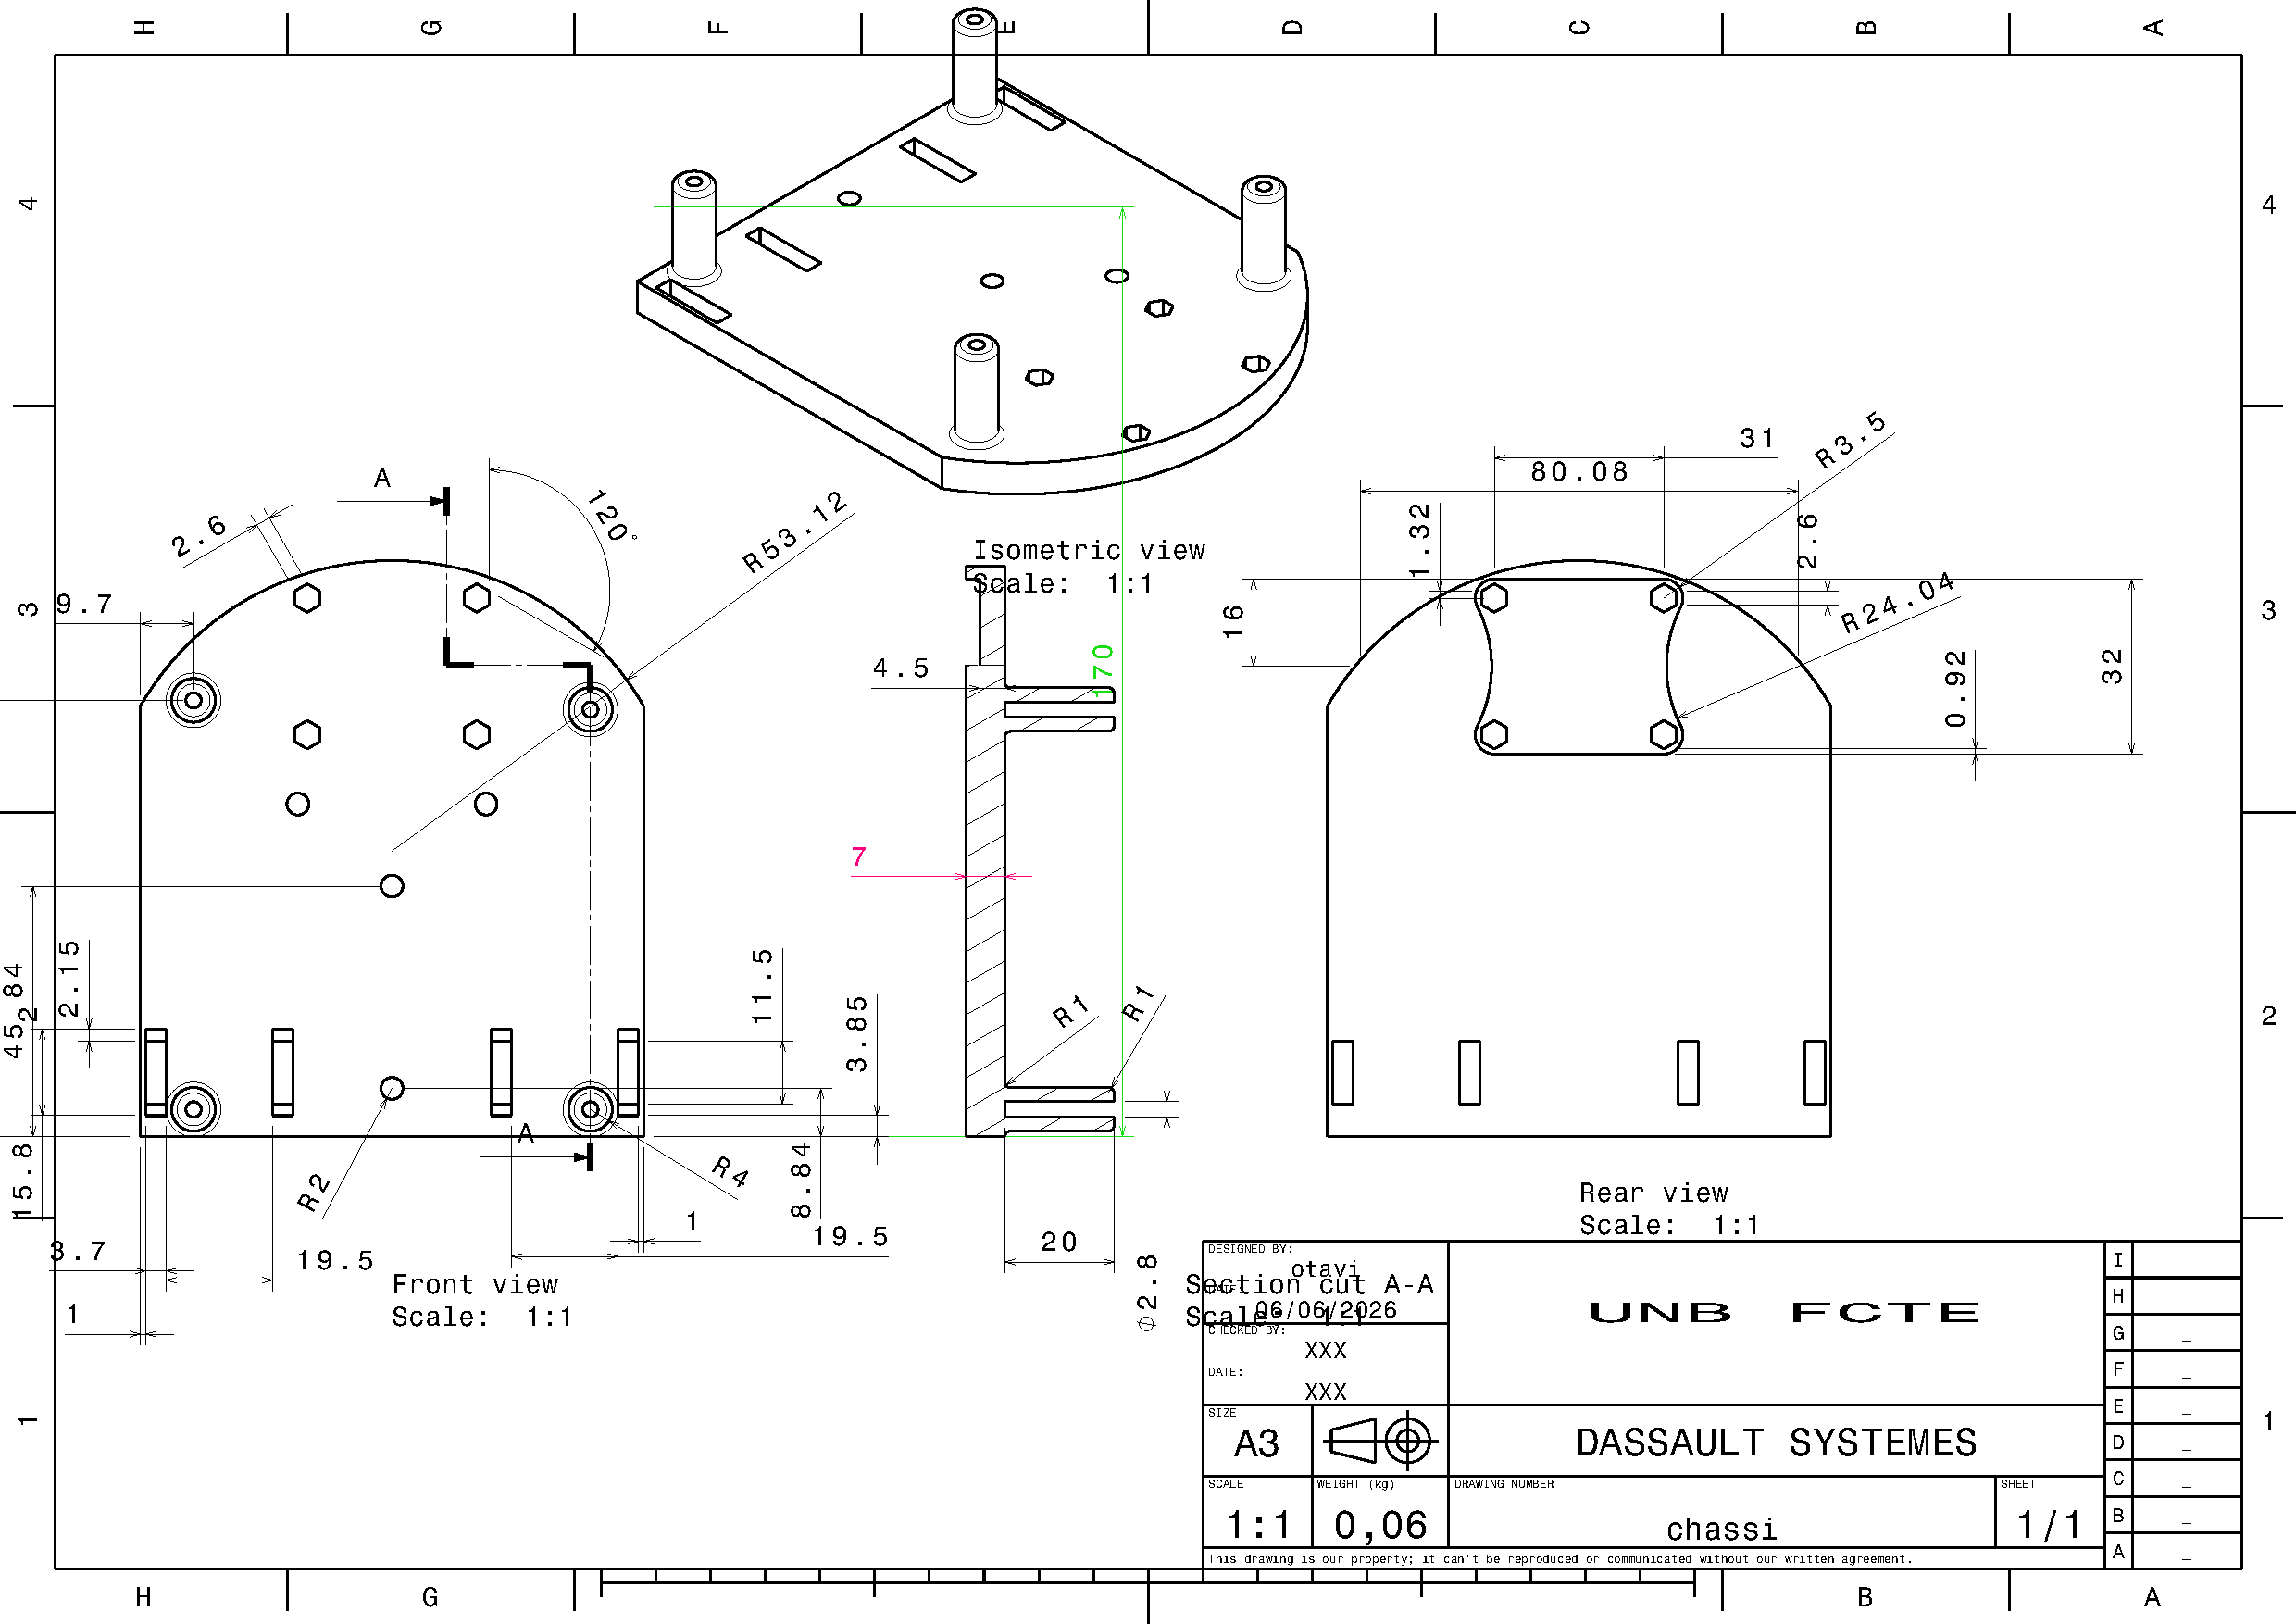
\includegraphics[width=0.60\linewidth]{figuras/1andar.pdf}
    \caption{Prancha técnica do segundo protótipo — primeiro andar: vistas frontal, traseira, isométrica e corte A-A (escala 1:1, peso 0{,}06\,kg).}
    \label{fig:chassi_draw_1andar}
\end{figure}

\begin{figure}[htbp]
    \centering
    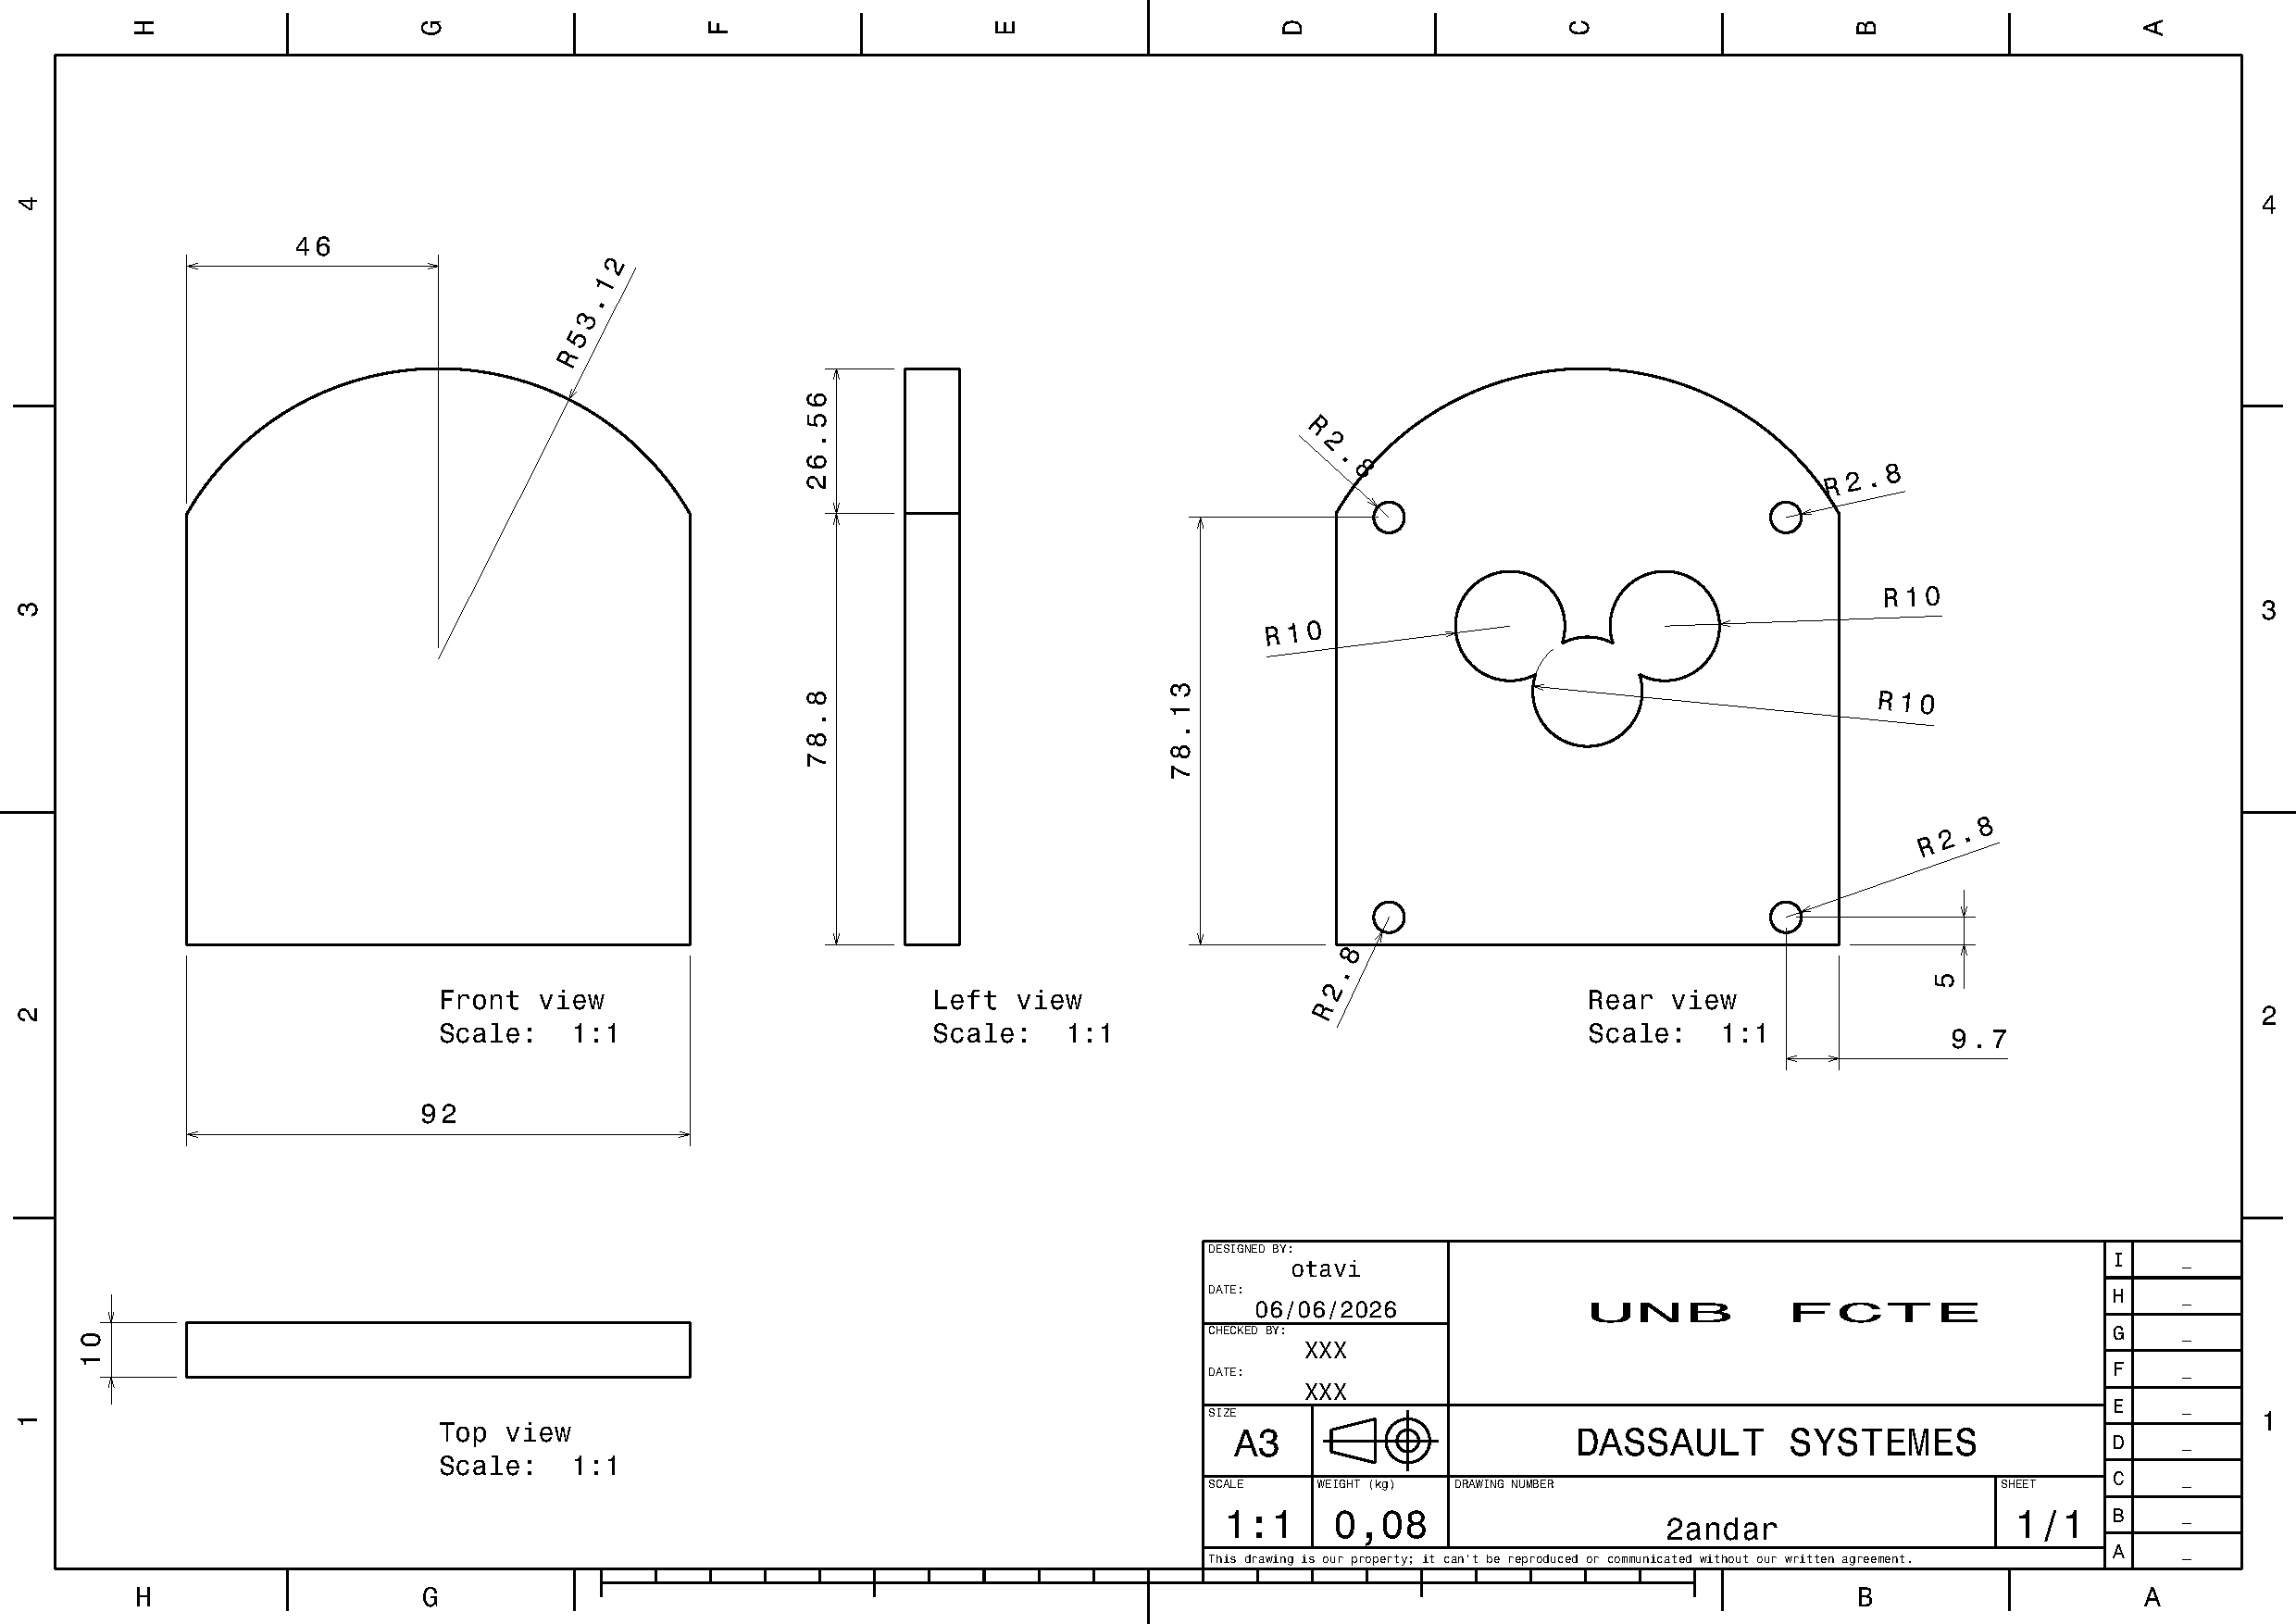
\includegraphics[width=0.60\linewidth]{figuras/2ANDAR.pdf}
    \caption{Prancha técnica do segundo protótipo — segundo andar: vistas frontal, lateral, traseira e superior (escala 1:1, peso 0{,}08\,kg).}
    \label{fig:chassi_draw_2andar}
\end{figure}



% \textcolor{red}{Apêndices e anexos são materiais complementares ao texto que só devem ser incluídos quando forem imprescindíveis à compreensão deste:}

% %%% https://www.codecogs.com/latex/eqneditor.php?lang=pt-br
% % \begin{equation}
% %     \alpha = \sum_{i=0}^{\infty}{a_i x^i}
% % \end{equation}

% % \begin{equation}
% %     \beta = \sum_{i=0}^{\infty}{a_i x^{2\pi i}\frac{\partial^2 }{\partial x^2}}f(xi)
% % \end{equation}

% \textcolor{red}{
% \begin{itemize}
%     \item Apêndices são textos elaborados pelo autor a fim de complementar sua argumentação.
%     \item Anexos são os documentos não elaborados pelo autor, que servem de fundamentação, comprovação ou ilustração, como mapas, leis, estatutos etc.
% \end{itemize}}

% \textcolor{red}{\textbf{Texto do primeiro apêndice.}}

\chapter{Esquemáticos Completos de Hardware}
\label{apendice_esquematicos_hw}

\begin{figure}[H]
    \centering
    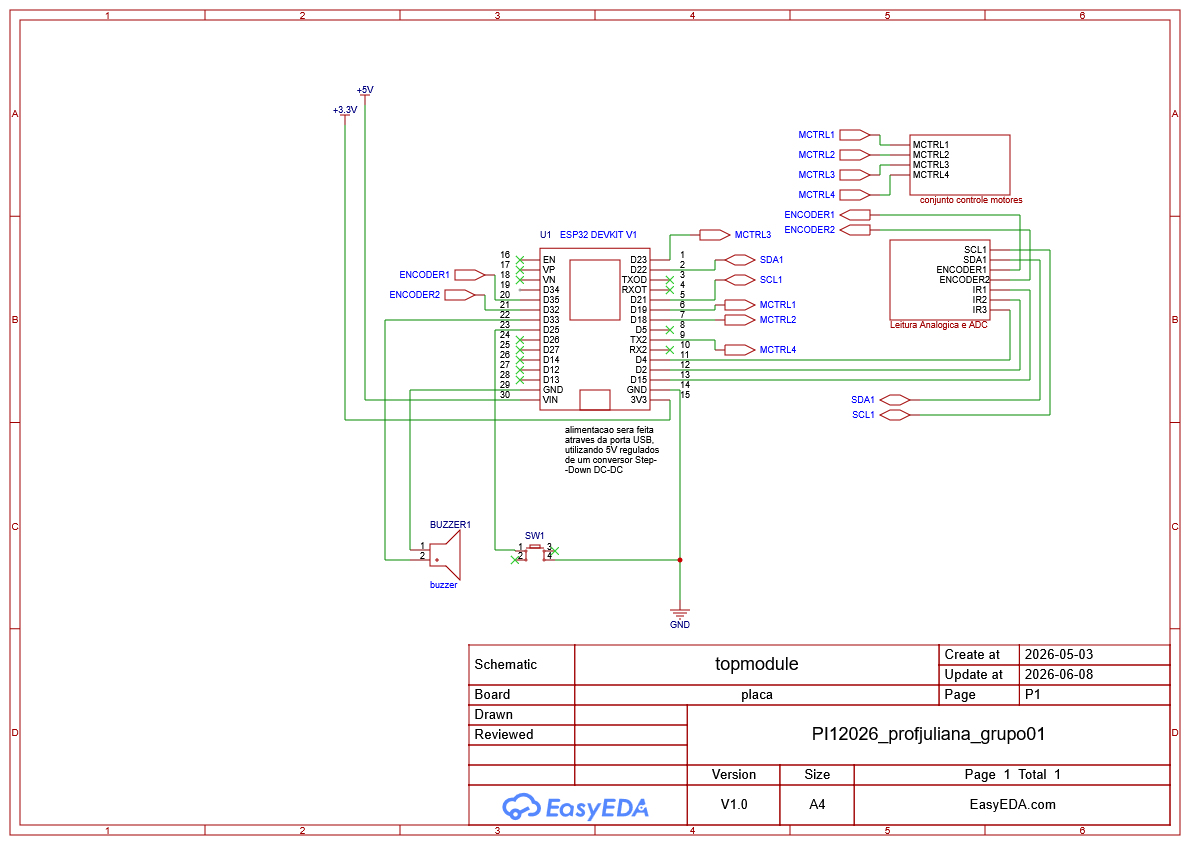
\includegraphics[width=0.8\linewidth]{figuras/SCH_topmodule_1-P1_2026-06-08.png}
    \caption{Representação da Ligação dos Componentes no Microcontrolador}
    \label{fig:esq_topmodule}
\end{figure}

\begin{figure}[H]
    \centering
    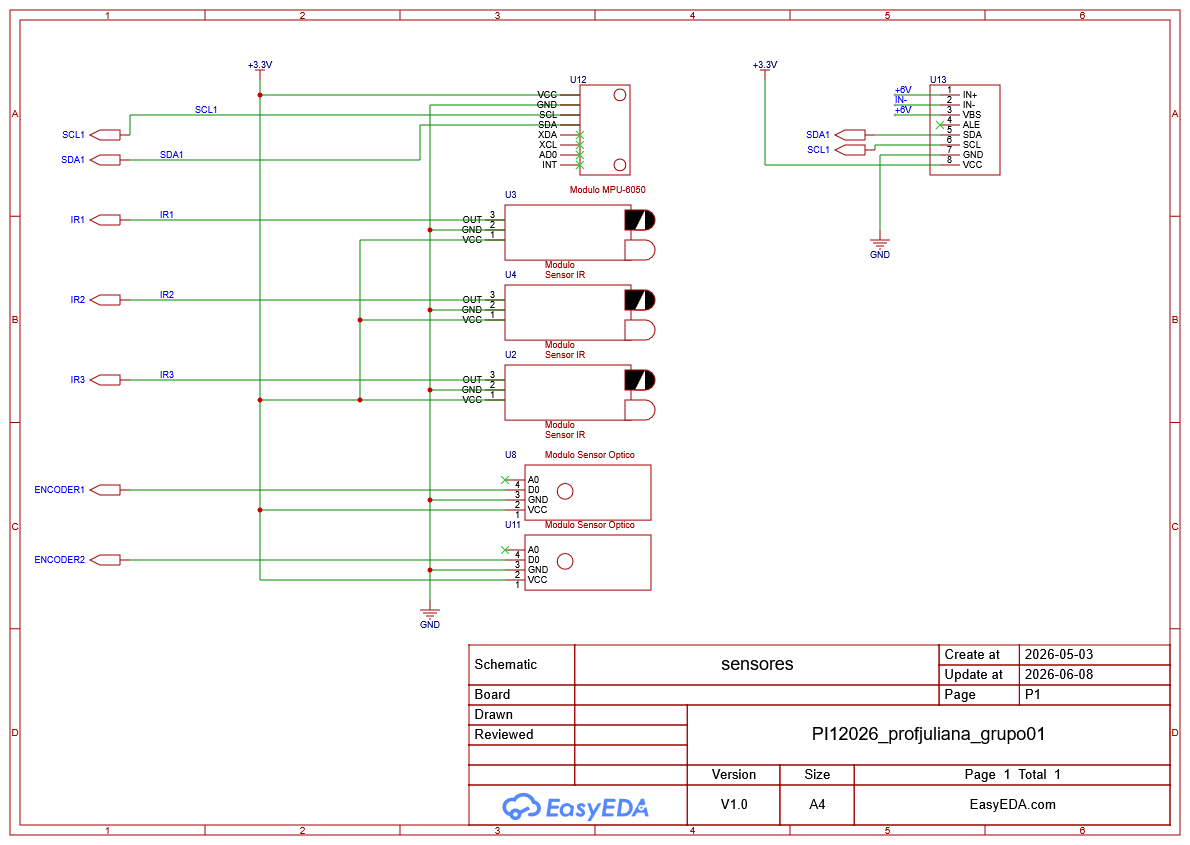
\includegraphics[width=0.8\linewidth]{figuras/SCH_sensores_1-P1_2026-06-08.png}
    \caption{Representação Esquemática dos Sensores}
    \label{fig:esq_sensores}
\end{figure}

\begin{figure}[H]
    \centering
    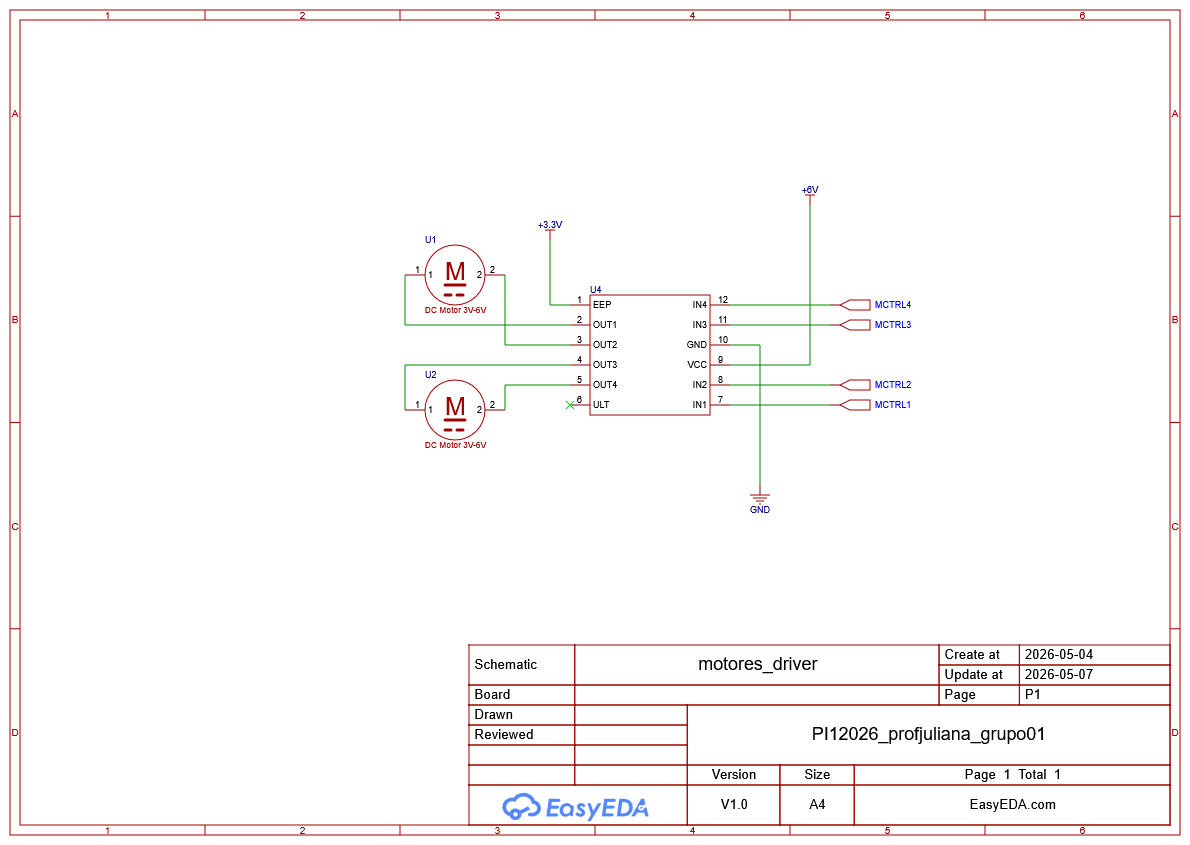
\includegraphics[width=0.8\linewidth]{figuras/SCH_motores_driver_1-P1_2026-06-08.png}
    \caption{Representação Esquemática do Driver e Motores}
    \label{fig:esq_motores}
\end{figure}

\begin{figure}[H]
    \centering
    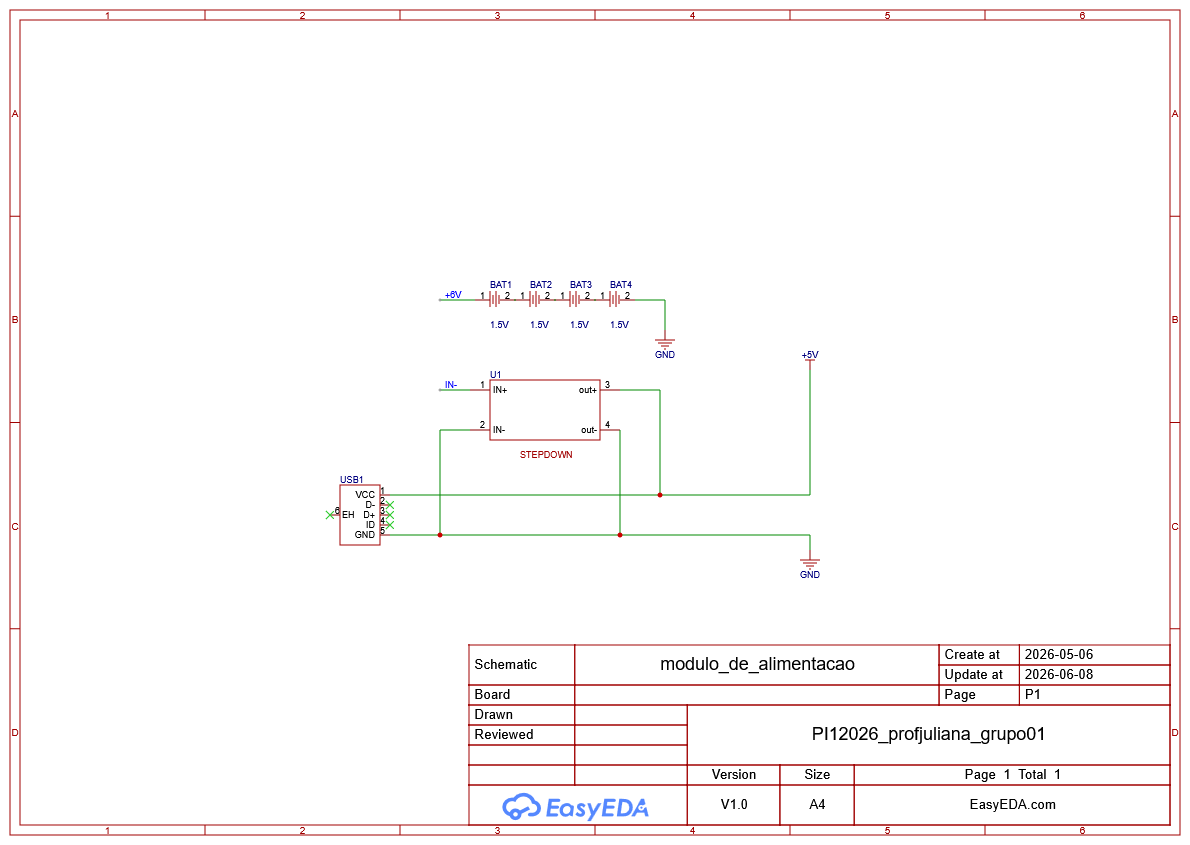
\includegraphics[width=0.8\linewidth]{figuras/SCH_modulo_de_alimentacao_1-P1_2026-06-08.png}
    \caption{Representação Esquemática da Alimentação do \textit{Micromouse}}
    \label{fig:esq_alimentacao}
\end{figure}

\chapter{Evidências dos Testes de Hardware}
\label{apendice_evidencias_testes_hardware}

Este apêndice reúne os registros do monitor serial utilizados para comprovar os
testes de bancada do módulo de \textit{hardware}, incluindo validação de
encoders, odometria e consumo elétrico do conjunto de motores e sensores.

\begin{figure}[H]
    \centering
    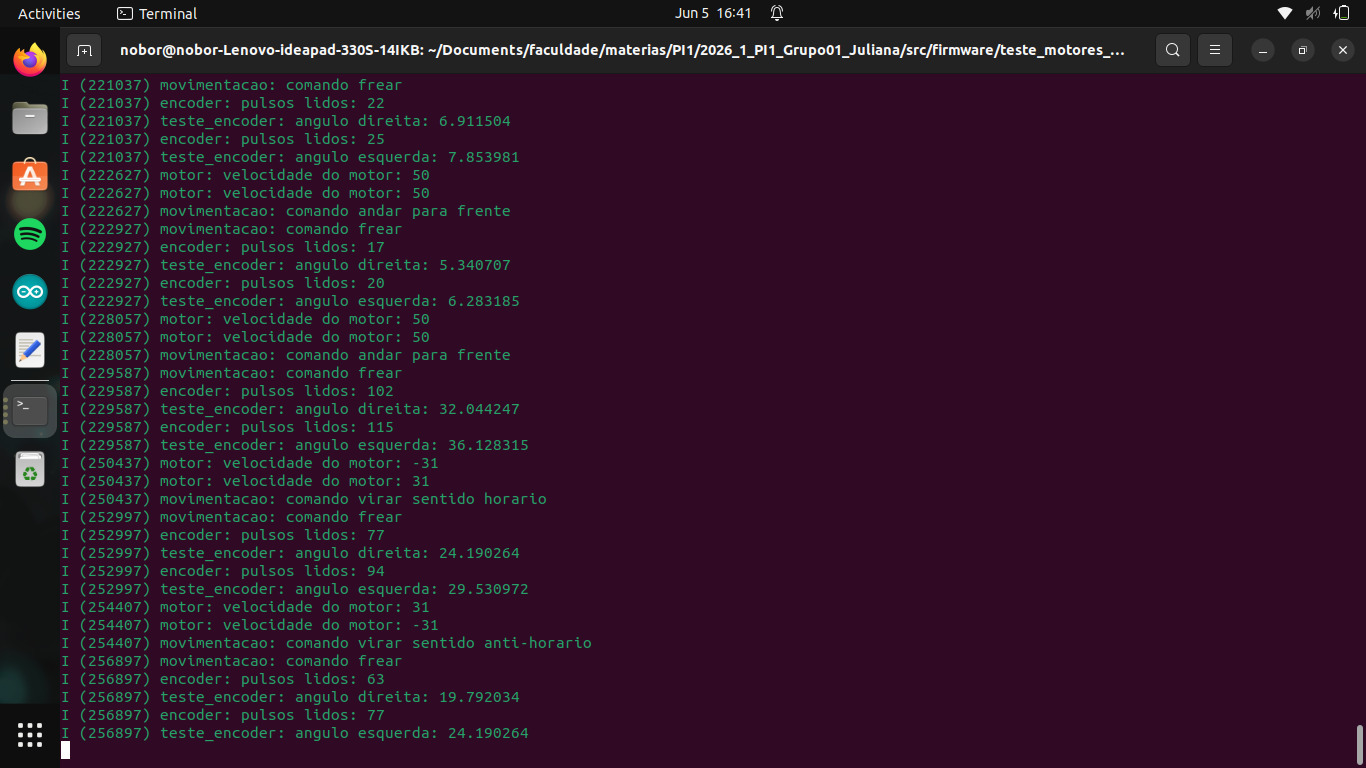
\includegraphics[width=\textwidth, keepaspectratio]{figuras/teste_valida_dados_encoder.jpeg}
    \caption{Validação dos dados dos encoders durante comandos de avanço, frenagem e giro, com registro de pulsos lidos e ângulos calculados para os lados direito e esquerdo.}
    \label{fig:teste_valida_dados_encoder}
\end{figure}

\begin{figure}[H]
    \centering
    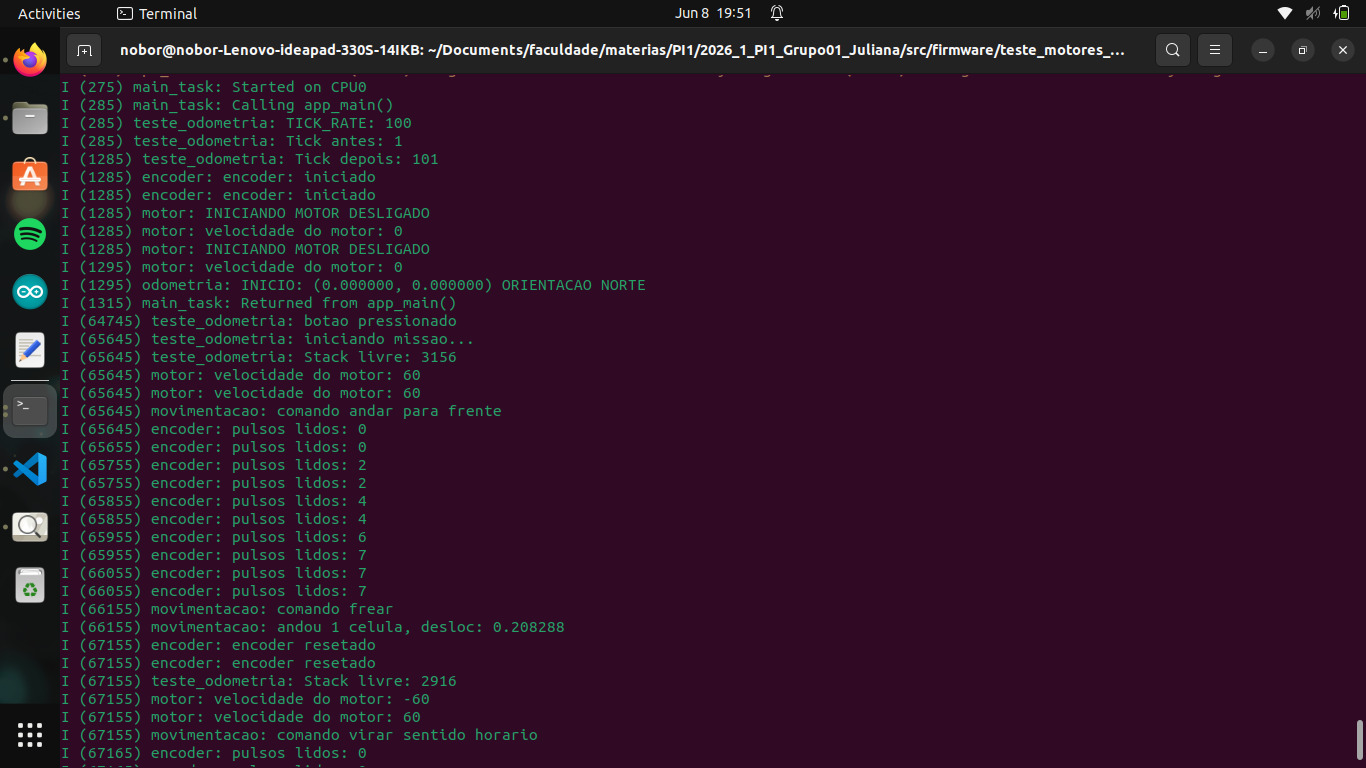
\includegraphics[width=\textwidth, keepaspectratio]{figuras/teste_odometria_1.jpeg}
    \caption{Primeira parte do teste de odometria, com inicialização do sistema, avanço de uma célula e início da leitura de pulsos dos encoders.}
    \label{fig:teste_odometria_1}
\end{figure}

\begin{figure}[H]
    \centering
    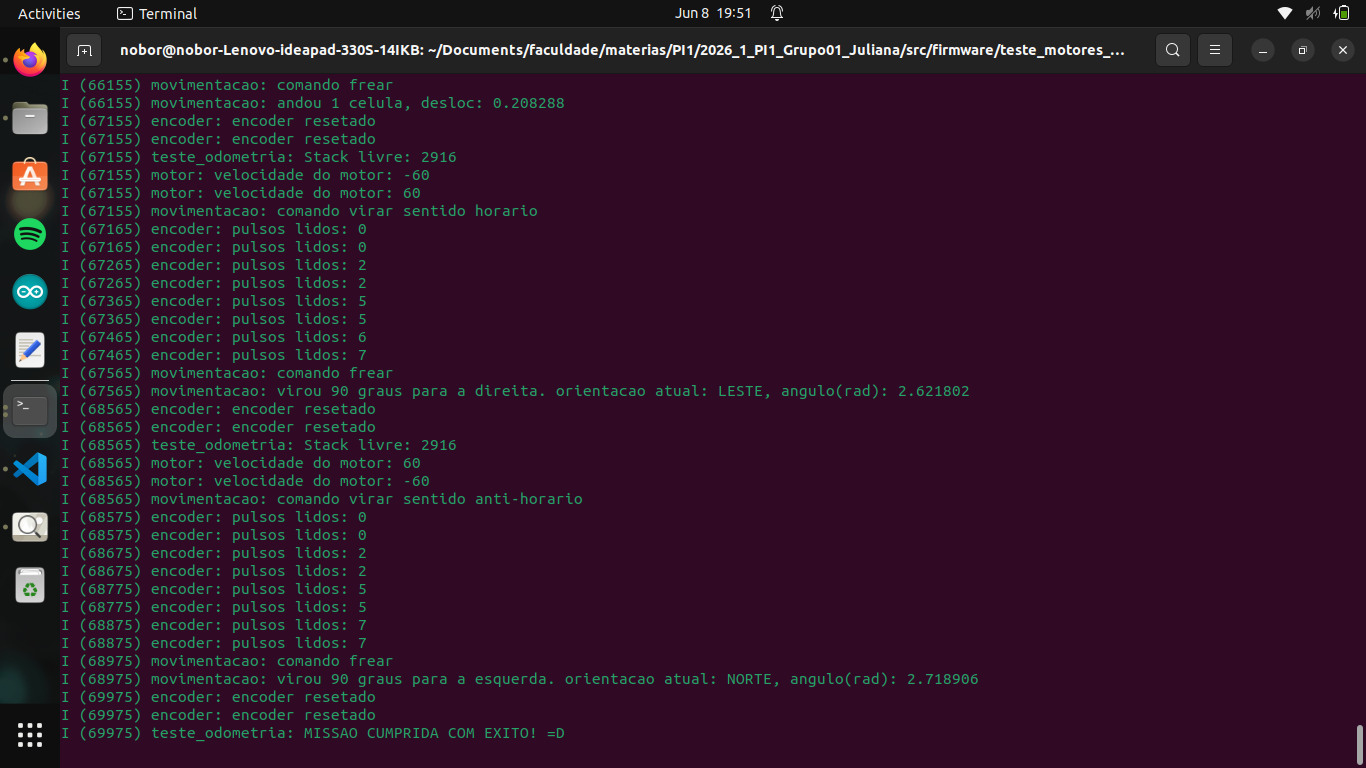
\includegraphics[width=\textwidth, keepaspectratio]{figuras/teste_odometria_2.jpeg}
    \caption{Segunda parte do teste de odometria, evidenciando giros de $90^\circ$, atualização da orientação do robô e conclusão do ensaio com sucesso.}
    \label{fig:teste_odometria_2}
\end{figure}

\begin{figure}[H]
    \centering
    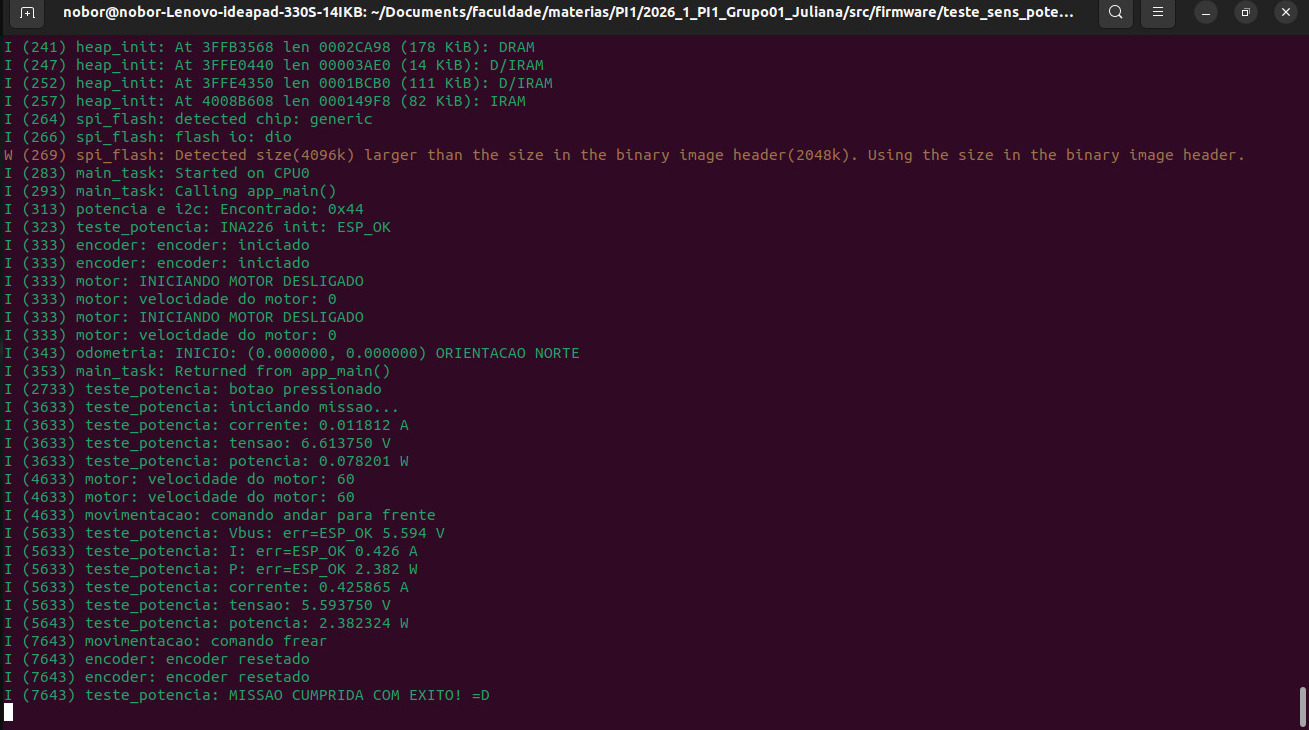
\includegraphics[width=\textwidth, keepaspectratio]{figuras/teste_sensor_potencia_motores_sem_esforço.jpeg}
    \caption{Teste do sensor de potência com o carrinho suspenso, no qual os motores giram sem oposição do piso, registrando tensão, corrente e potência pelo INA226.}
    \label{fig:teste_potencia_motores_sem_esforco}
\end{figure}

\begin{figure}[H]
    \centering
    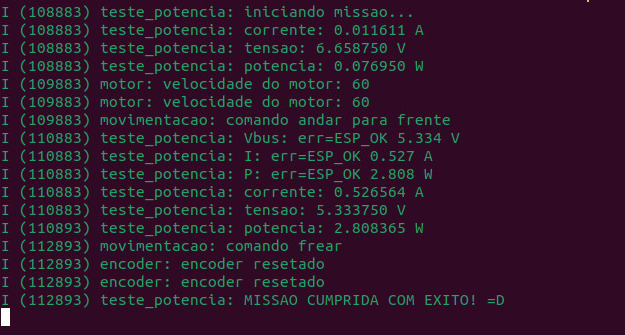
\includegraphics[width=\textwidth, keepaspectratio]{figuras/teste_sensor_potencia_motores_com_esforço.jpeg}
    \caption{Teste do sensor de potência com o carrinho apoiado no chão, no qual os motores precisam vencer a inércia do robô para iniciar o deslocamento.}
    \label{fig:teste_potencia_motores_com_esforco}
\end{figure}

% \textcolor{red}{Apêndices e anexos são materiais complementares ao texto que só devem ser incluídos quando forem imprescindíveis à compreensão deste:}

% \textcolor{red}{
% \begin{itemize}
%     \item Apêndices são textos elaborados pelo autor a fim de complementar sua argumentação.
%     \item Anexos são os documentos não elaborados pelo autor, que servem de fundamentação, comprovação ou ilustração, como mapas, leis, estatutos etc.
% \end{itemize}}

% \textcolor{red}{\textbf{Texto do segundo apêndice.}}

\chapter{Protótipos de Telas do Sistema Web}
\label{apendice_prototipos}

\begin{figure}[H]
    \centering
    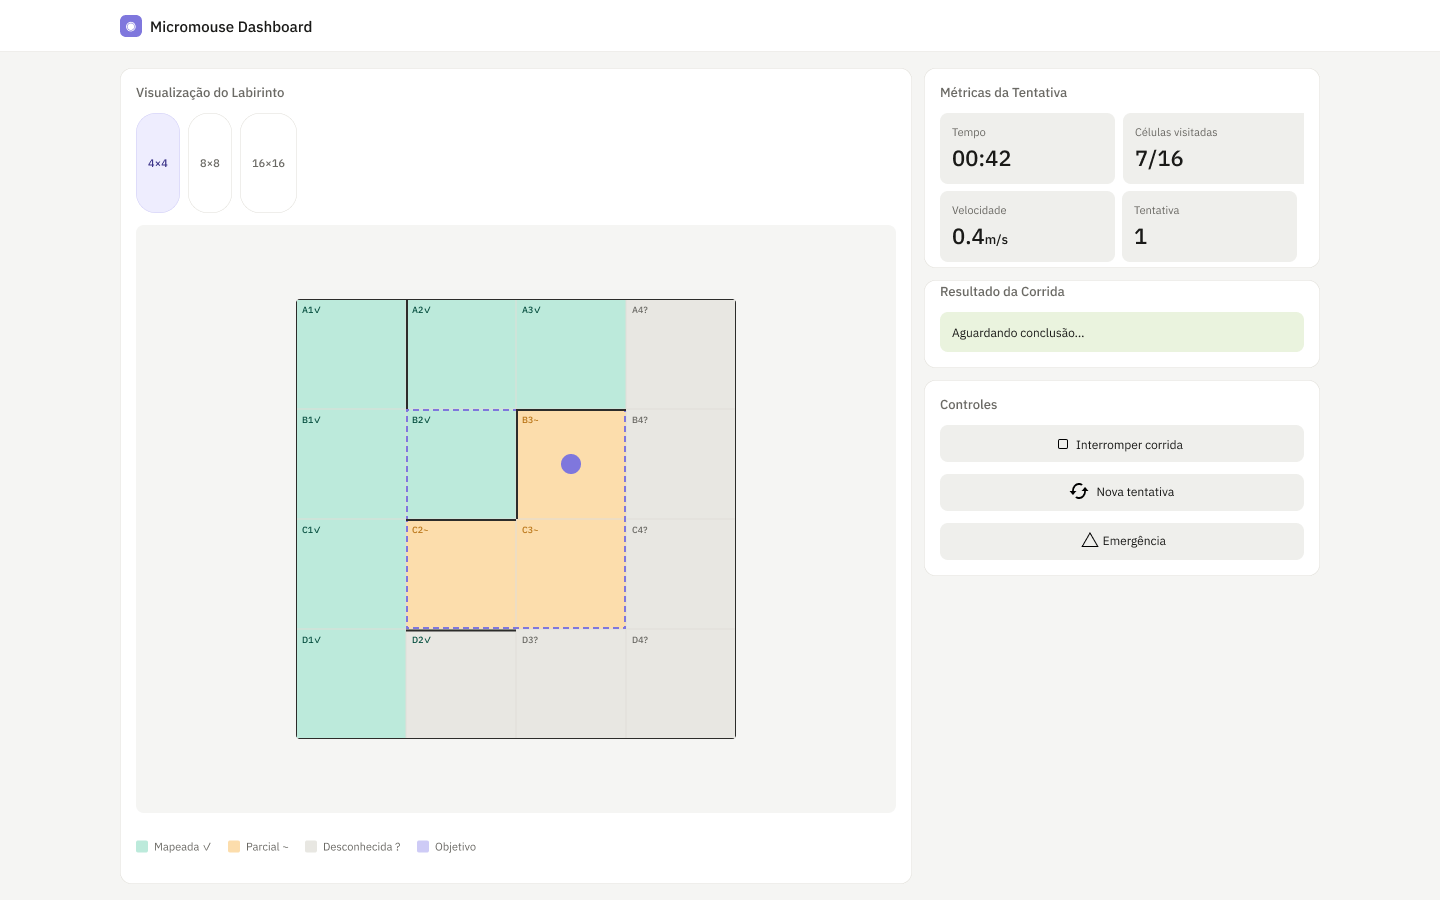
\includegraphics[width=0.8\textwidth, keepaspectratio]{figuras/HU01–Execução autônoma.png}
    \caption{Protótipo da HU01 – Resolução autônoma do labirinto.}
    \label{fig:execucaoautonoma_fig}
\end{figure}

\begin{figure}[H]
    \centering
    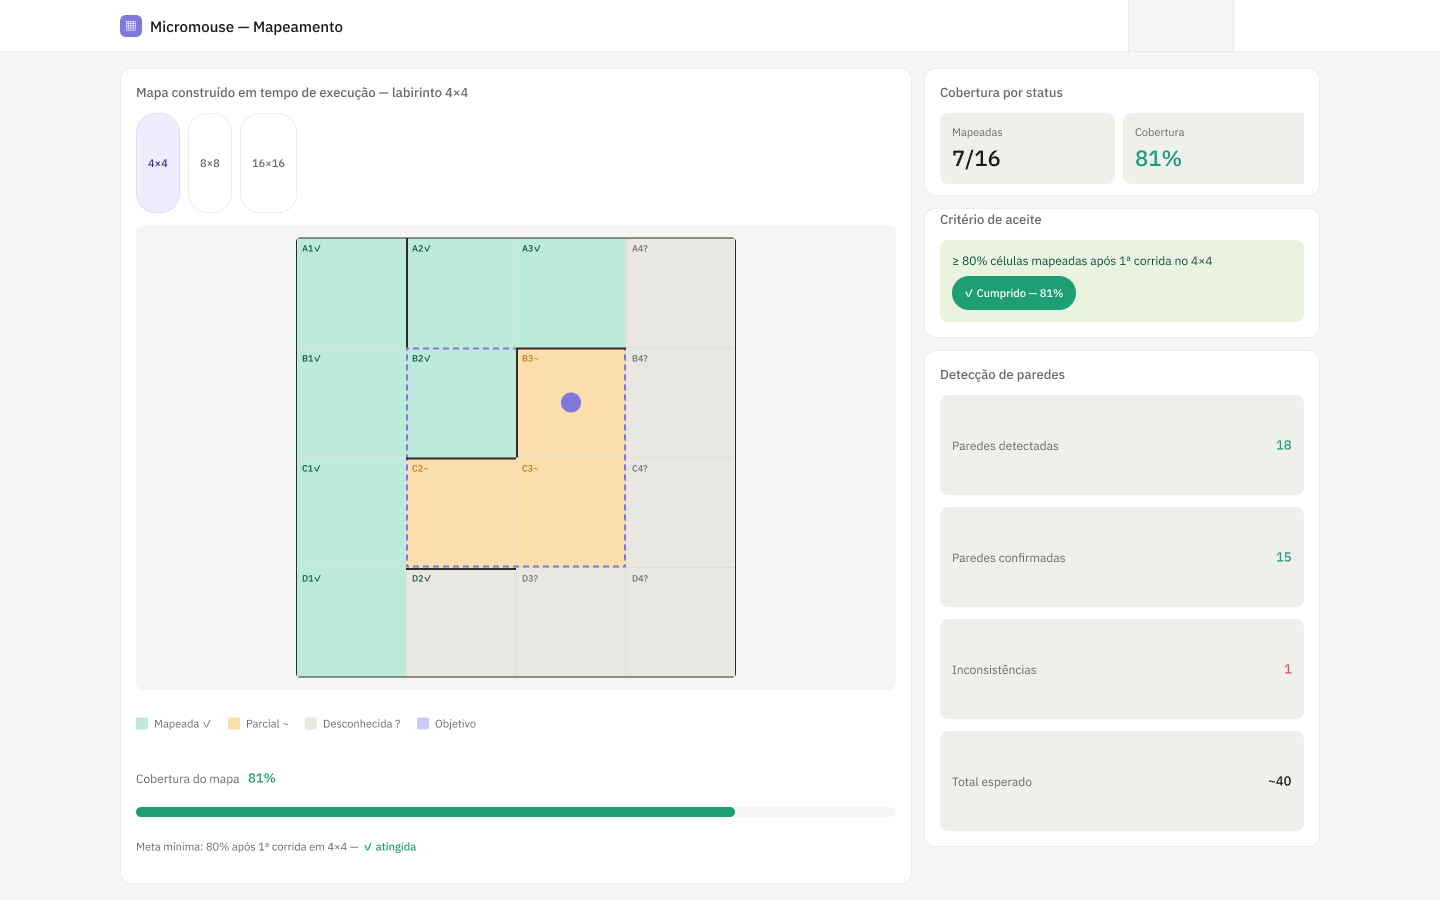
\includegraphics[width=0.8\textwidth, keepaspectratio]{figuras/HU02–Mapeamento incremental.png}
    \caption{Protótipo da HU02 – Mapeamento incremental do labirinto.}
    \label{fig:mapeamento_fig}
\end{figure}

\begin{figure}[H]
    \centering
    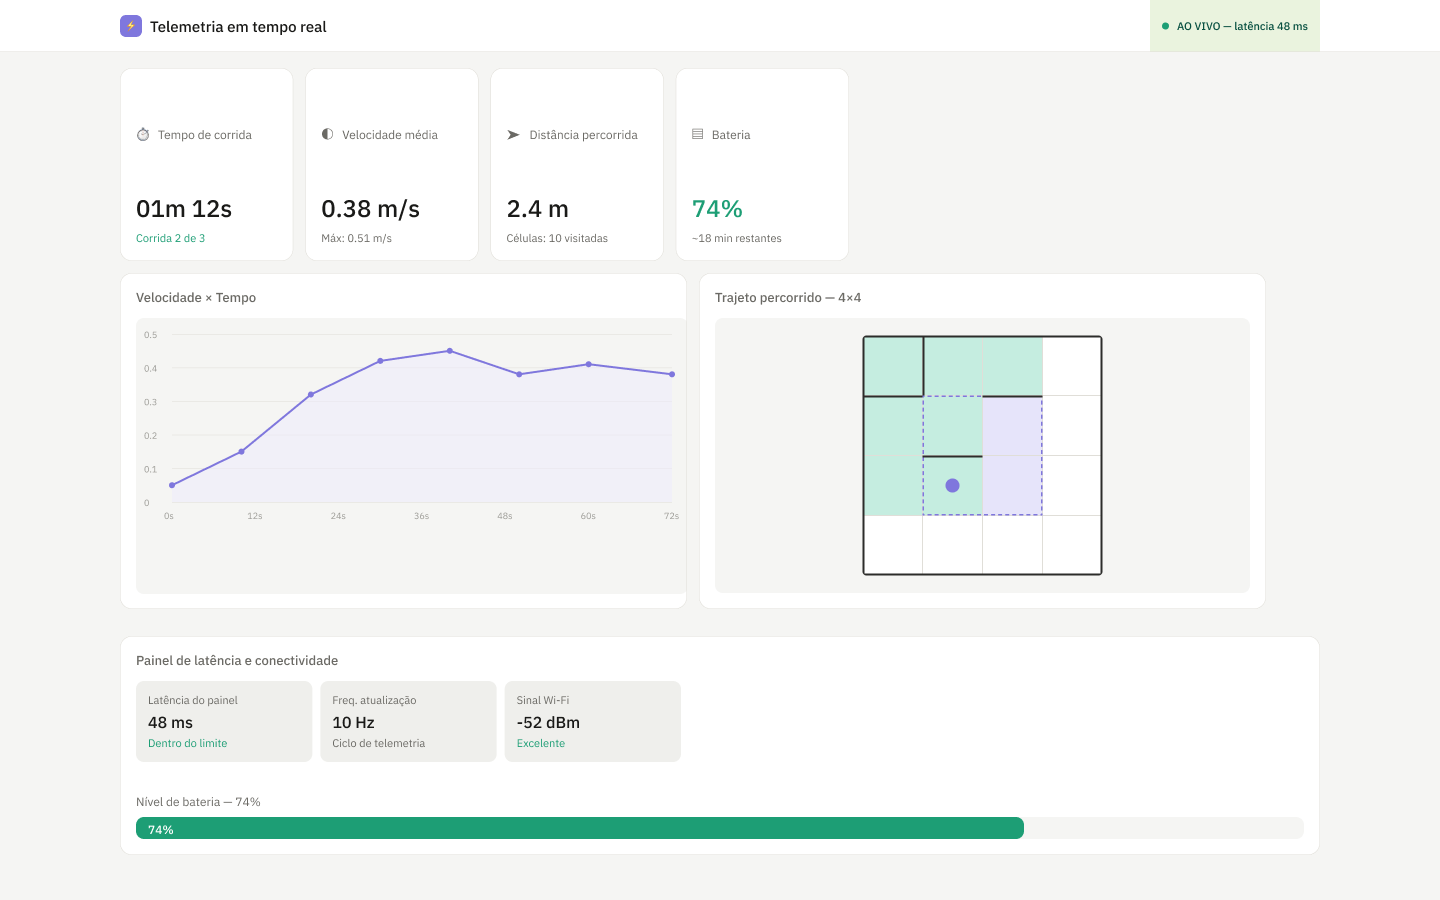
\includegraphics[width=0.95\textwidth, keepaspectratio]{figuras/HU03–Telemetria em tempo real.png}
    \caption{Protótipo da HU03 – Telemetria em tempo real.}
    \label{fig:telemetria_fig}
\end{figure}

\begin{figure}[H]
    \centering
    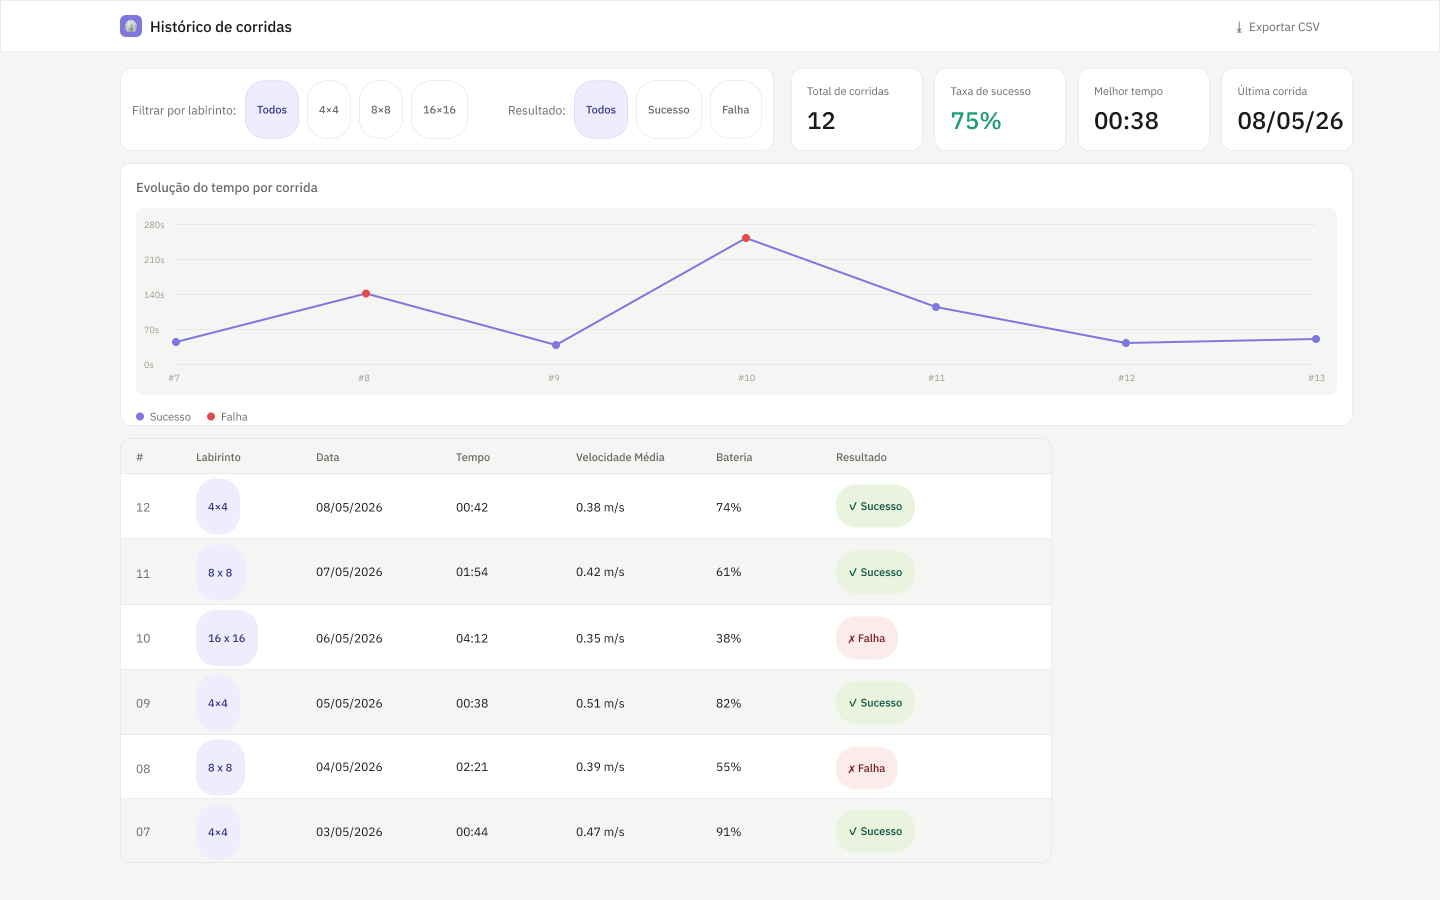
\includegraphics[width=0.8\textwidth, keepaspectratio]{figuras/HU04–Histórico de corridas.png}
    \caption{Protótipo da HU04 – Persistência e consulta de histórico.}
    \label{fig:historicocorridas_fig}
\end{figure}

\begin{figure}[H]
    \centering
    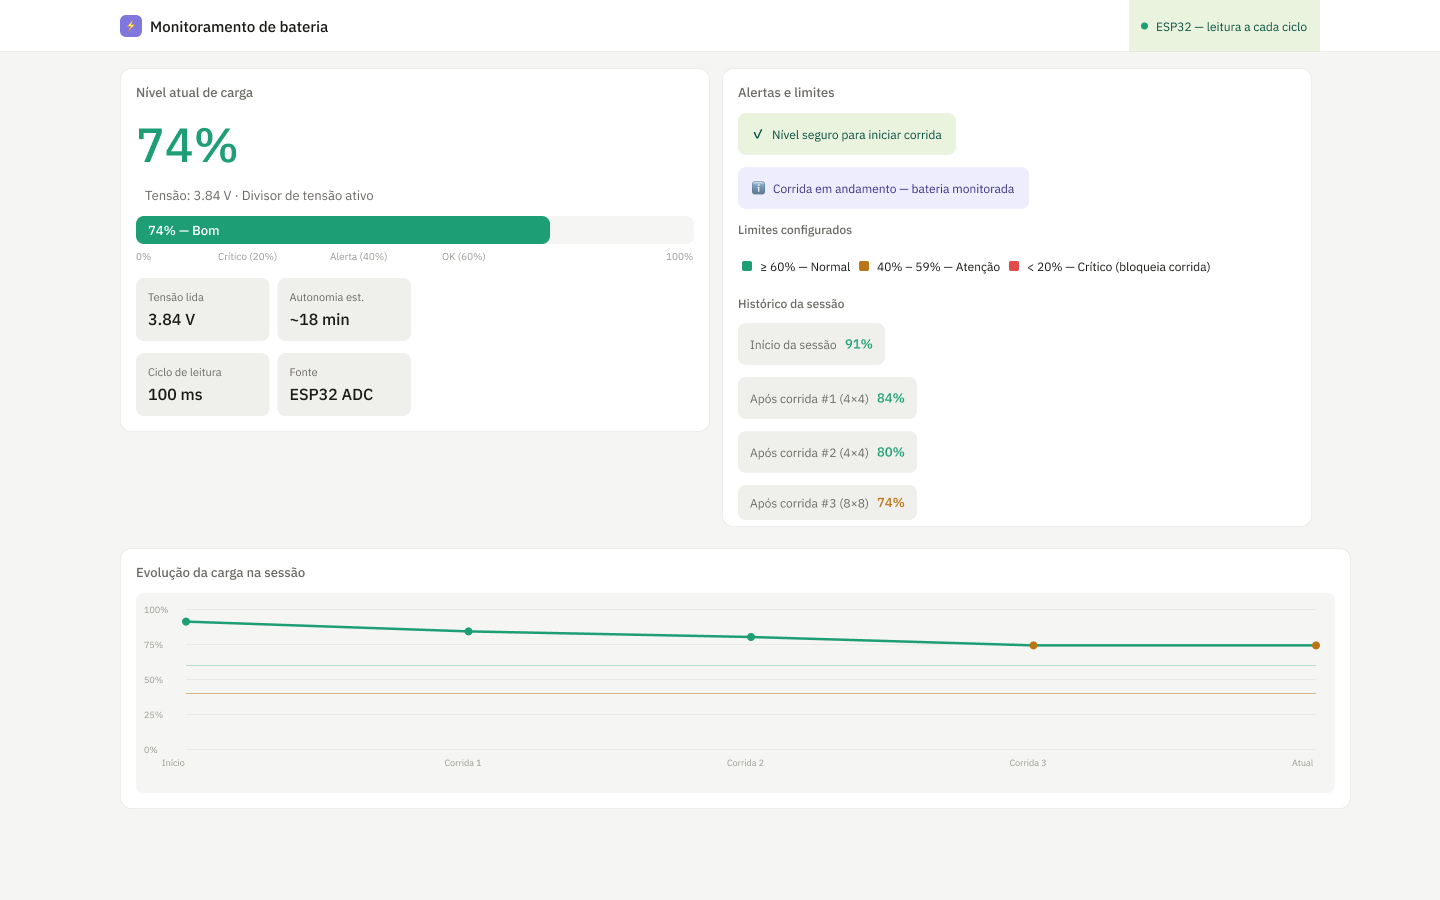
\includegraphics[width=0.8\textwidth, keepaspectratio]{figuras/HU05–Monitoramento de bateria.png}
    \caption{Protótipo da HU05 – Monitoramento de bateria.}
    \label{fig:monitoramentobateria_fig}
\end{figure}

\begin{figure}[H]
    \centering
    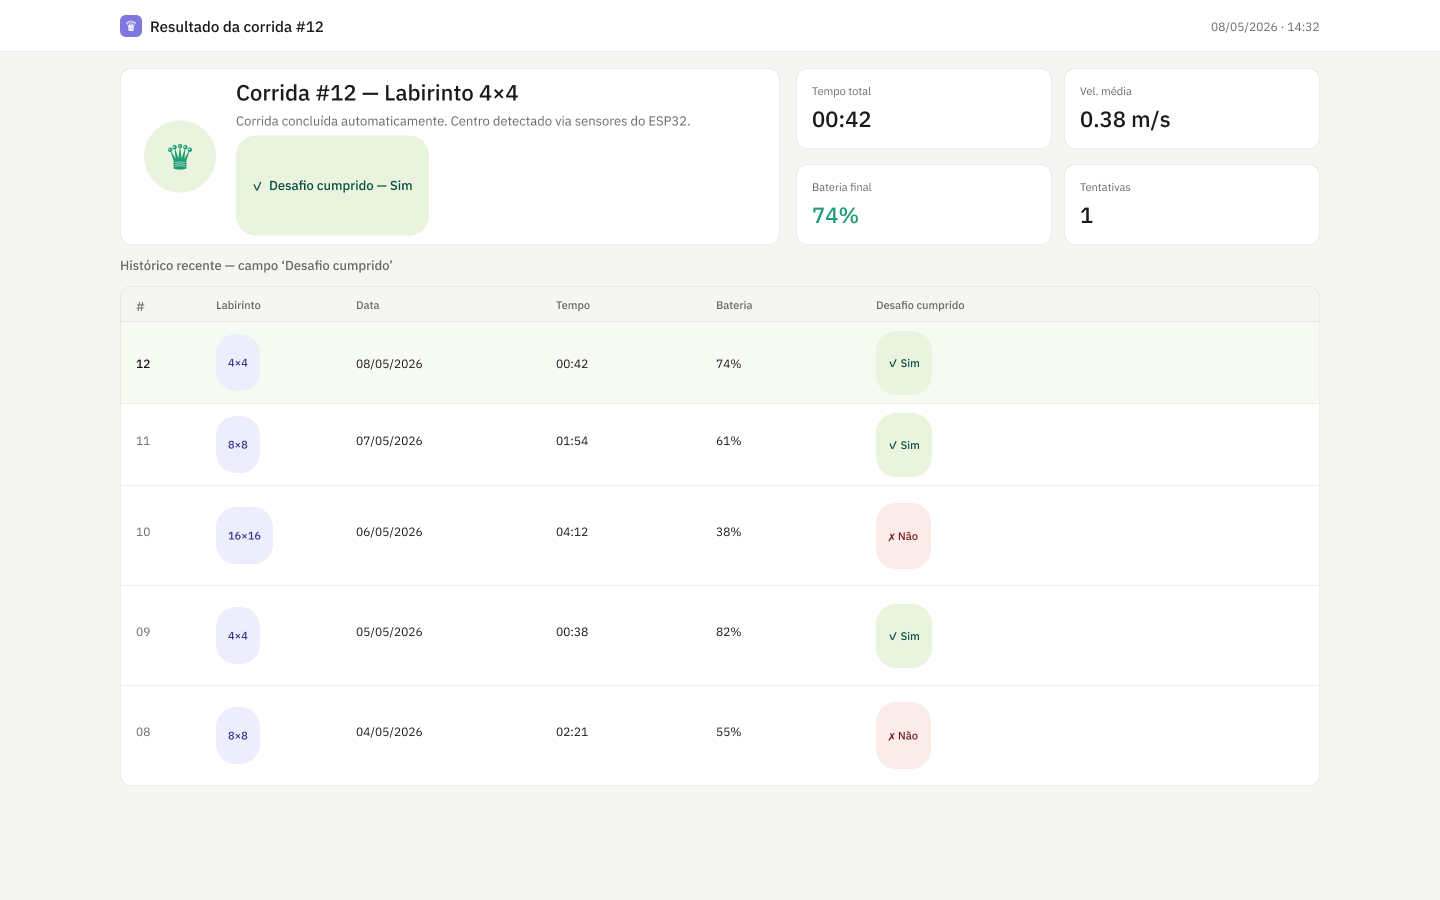
\includegraphics[width=0.8\textwidth, keepaspectratio]{figuras/HU06–Desafio cumprido.png}
    \caption{Protótipo da HU06 – Indicador de desafio cumprido.}
    \label{fig:desafiocumprido_fig}
\end{figure}


\begin{landscape}
\chapter{Roteiro Detalhado de Testes Funcionais}
\label{apendice_roteiro_detalhado}

\begin{small}
\begin{longtable}{|p{1.2cm}|p{3cm}|p{3.5cm}|p{4cm}|p{5.5cm}|p{4cm}|}
    \caption{Roteiro de testes funcionais do sistema Micromouse.}
    \label{tab:testes-funcionais} \\
    \hline
    \textbf{Código} & \textbf{Nome} & \textbf{Objetivo} & \textbf{Pré-condições} & \textbf{Procedimento} & \textbf{Resultado esperado} \\ \hline
    \endfirsthead

    \multicolumn{6}{c}%
    {{\bfseries Tabela \thetable{} -- continuação da página anterior}} \\
    \hline
    \textbf{Código} & \textbf{Nome} & \textbf{Objetivo} & \textbf{Pré-condições} & \textbf{Procedimento} & \textbf{Resultado esperado} \\ \hline
    \endhead

    \hline \multicolumn{6}{|r|}{{Continua na próxima página...}} \\ \hline
    \endfoot

    \hline
    \endlastfoot

    TF01 & Resolução autônoma em labirinto 4×4 (HU01, RF01, RF03) &
    Validar a execução completa da navegação autônoma até o centro do labirinto, sem qualquer intervenção humana. &
    Labirinto 4×4 montado conforme as dimensões oficiais; bateria com carga $\geq$ 80\%; firmware com o algoritmo Flood Fill gravado; robô posicionado na célula de partida orientado para o norte. &
    1) Ligar o robô; 2) acionar o botão de início; 3) acompanhar a execução até a parada autônoma; 4) inspecionar visualmente, ao final, se houve contato com paredes durante o trajeto. &
    Robô alcança a célula central em $\leq$ 60 s sem tocar nas paredes, sinaliza chegada (LED) e não houve qualquer interação humana durante a tentativa. \\ \hline

    TF02 & Mapeamento incremental de paredes (HU02, RF02, RF06) &
    Verificar que o firmware detecta e registra as paredes do labirinto à medida que explora, construindo o mapa em tempo de execução. &
    TF01 executado com sucesso; labirinto 4×4 com layout previamente conhecido pela equipe; canal de log (serial ou MQTT) ativo para extração do mapa. &
    1) Iniciar uma corrida no labirinto 4×4 conhecido; 2) ao final, extrair o mapa gerado (via log serial ou endpoint REST); 3) comparar o mapa célula a célula com o layout físico de referência. &
    Ao menos 80\% das células do labirinto 4×4 são corretamente mapeadas (critério da HU02), sem falsos positivos de parede registrados. \\ \hline

    TF03 & Telemetria em tempo real no painel web (HU03, RF09) &
    Verificar a atualização contínua de posição, tempo de corrida e nível de bateria no painel web, com latência aceitável. &
    Backend FastAPI e broker MQTT em execução; frontend acessível pelo navegador; robô (ou simulador) conectado à rede e publicando telemetria. &
    1) Abrir o painel web; 2) iniciar uma corrida (real ou simulada); 3) cronometrar o intervalo entre atualizações consecutivas exibidas; 4) confirmar que posição, tempo e bateria atualizam sem recarregar a página. &
    Os campos de posição, tempo e bateria são atualizados em intervalos $\leq$ 500\,ms durante toda a corrida (mínimo de 60\,s observados) e nenhuma recarga manual da página é necessária. \\ \hline

    TF04 & Persistência da corrida ao término (HU04) &
    Garantir que os dados finais de cada corrida concluída são gravados no banco e ficam disponíveis para consulta. &
    Backend e banco de dados (SQLite ou PostgreSQL) operacionais; tela de histórico acessível; corrida em execução prestes a terminar. &
    1) Concluir a corrida (chegada ao centro ou parada controlada); 2) aguardar o evento de fim; 3) acessar a tela de histórico; 4) inspecionar o registro mais recente. &
    Aparece um novo registro no histórico contendo, no mínimo, data/hora, duração, velocidade média, tamanho do labirinto e resultado, e o mesmo é recuperável via \texttt{GET /corridas}. \\ \hline

    TF05 & Filtro do histórico por tamanho de labirinto (HU04, UC12) &
    Verificar que o filtro de consulta exibe apenas corridas do tamanho de labirinto selecionado. &
    Banco de dados contendo ao menos uma corrida persistida para cada dimensão (4×4, 8×8 e 16×16); tela de histórico aberta. &
    1) Selecionar a opção ``4×4'' no filtro e conferir a lista; 2) repetir para ``8×8'' e ``16×16''; 3) limpar o filtro e conferir a lista completa. &
    Em cada seleção, apenas corridas da dimensão escolhida são exibidas; ao limpar o filtro, todas as corridas voltam a ser listadas. \\ \hline

    TF06 & Leitura do nível de bateria via divisor de tensão (HU05, RF08) &
    Validar a leitura analógica do divisor de tensão pelo ESP32 e a transmissão do percentual de carga para o painel web. &
    Chassi montado com o divisor de tensão conforme o esquemático; multímetro digital disponível como referência; firmware com módulo de monitoramento de bateria ativo; painel web aberto. &
    1) Medir a tensão real da bateria com o multímetro; 2) comparar com o percentual exibido no painel; 3) repetir a medição após 10\,min de operação contínua. &
    O percentual exibido no painel corresponde à leitura do multímetro com erro $\leq$ 5\% e diminui de forma monotônica ao longo do tempo de uso. \\ \hline

    TF07 & Indicador ``Desafio cumprido'' preenchido automaticamente (HU06) &
    Verificar que o sistema atribui automaticamente ``Sim'' ou ``Não'' ao campo ``Desafio cumprido'' com base na detecção da chegada ao centro. &
    Backend, frontend e firmware operacionais; lógica de detecção do centro habilitada; tela de histórico acessível. &
    Cenário A) realizar uma corrida em que o robô atinge o centro e, em seguida, consultar o histórico. Cenário B) interromper manualmente uma corrida antes da chegada e consultar o histórico. &
    Cenário A: o campo ``Desafio cumprido'' aparece como ``Sim'' para a corrida concluída. Cenário B: o mesmo campo aparece como ``Não'' para a corrida interrompida. \\ \hline

    TF08 & Detecção da chegada ao centro do labirinto (RF04, UC07) &
    Garantir que a chegada à célula central dispara o encerramento da corrida e o envio das estatísticas finais ao backend. &
    Labirinto 4×4 montado; firmware com lógica de detecção de centro; comunicação MQTT ativa entre robô e backend. &
    1) Posicionar o robô na célula de partida; 2) iniciar a corrida; 3) observar o comportamento ao atingir a célula central; 4) confirmar nos logs e via API REST o registro do evento de fim de corrida. &
    Ao alcançar a célula central, o robô para imediatamente, publica uma mensagem MQTT com as estatísticas finais e a corrida é registrada como concluída no histórico. \\ \hline

\end{longtable}
\end{small}
\end{landscape}

\chapter{Evidências de Testes e Cobertura de Código}
\label{apendice_evidencias_testes}

Este apêndice reúne as evidências de execução das suítes de testes automatizados e
de cobertura de código-fonte do \textit{software}, geradas pelo \textit{pipeline} de
Integração Contínua e referenciadas na Seção~\ref{sec:testes_software}.

\begin{figure}[H]
    \centering
    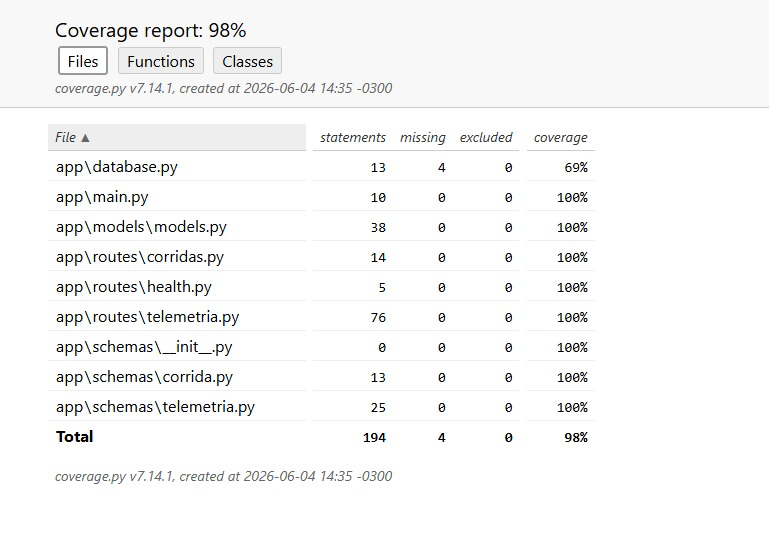
\includegraphics[width=0.85\textwidth, keepaspectratio]{figuras/cobertura_backend.png}
    \caption{Relatório de cobertura do \textit{backend} (\texttt{pytest-cov}): $98\%$ de
    cobertura total, acima do mínimo de $70\%$.}
    \label{fig:cobertura_backend}
\end{figure}

\begin{figure}[H]
    \centering
    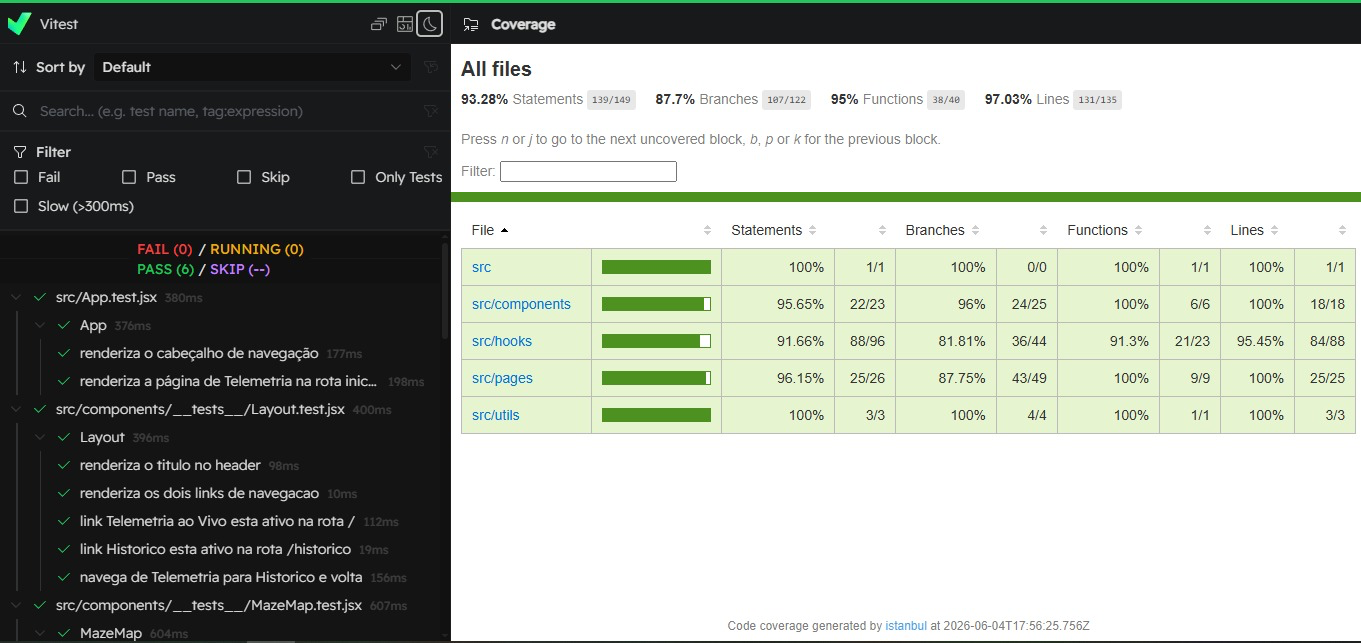
\includegraphics[width=\textwidth, keepaspectratio]{figuras/cobertura_frontend.png}
    \caption{Relatório de cobertura do \textit{frontend} (\texttt{Vitest}): $93{,}28\%$ de
    \textit{statements} e $97{,}03\%$ de linhas, acima do mínimo de $70\%$.}
    \label{fig:cobertura_frontend}
\end{figure}

\begin{figure}[H]
    \centering
    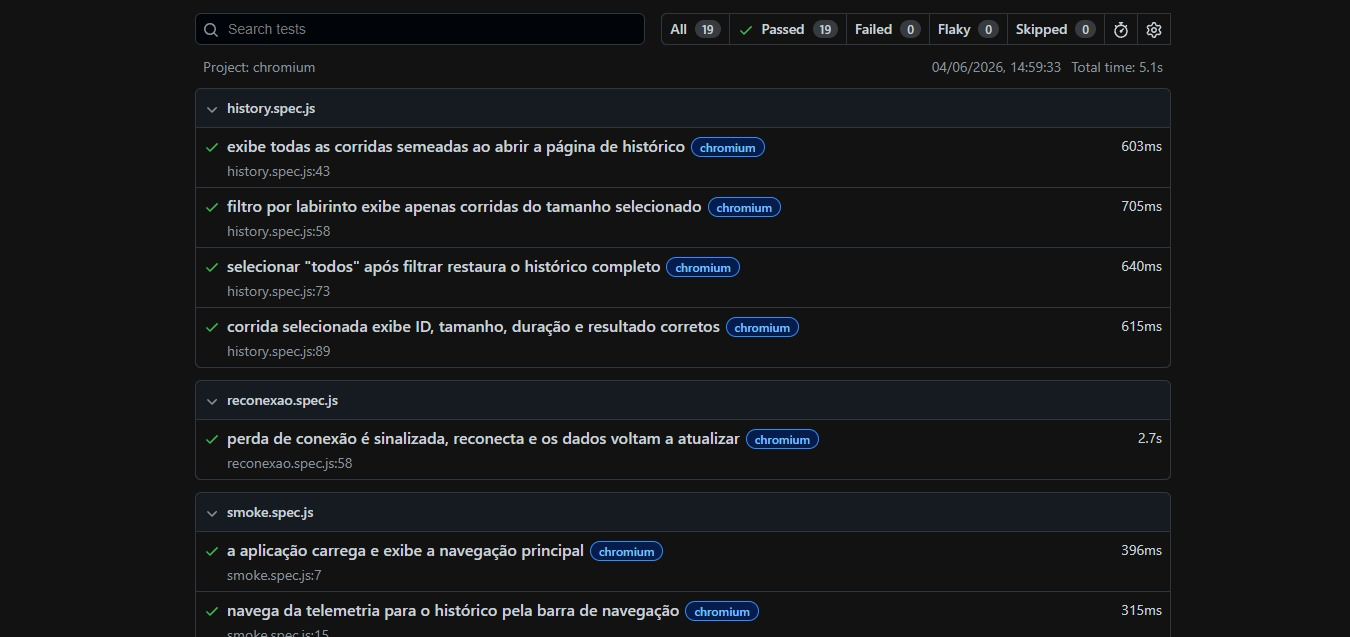
\includegraphics[width=\textwidth, keepaspectratio]{figuras/e2e_playwright.png}
    \caption{Relatório dos testes de sistema E2E (\texttt{Playwright}): 19 casos
    aprovados, distribuídos nas quatro suítes funcionais.}
    \label{fig:e2e_playwright}
\end{figure}

% \textcolor{red}{Apêndices e anexos são materiais complementares ao texto que só devem ser incluídos quando forem imprescindíveis à compreensão deste:}

% \textcolor{red}{
% \begin{itemize}
%     \item Apêndices são textos elaborados pelo autor a fim de complementar sua argumentação.
%     \item Anexos são os documentos não elaborados pelo autor, que servem de fundamentação, comprovação ou ilustração, como mapas, leis, estatutos etc.
% \end{itemize}}

% \textcolor{red}{\textbf{Texto do segundo apêndice.}}

\end{apendicesenv}